% CVPR 2023 Paper Template
% based on the CVPR template provided by Ming-Ming Cheng (https://github.com/MCG-NKU/CVPR_Template)
% modified and extended by Stefan Roth (stefan.roth@NOSPAMtu-darmstadt.de)

\documentclass[10pt,twocolumn,letterpaper]{article}

%%%%%%%%% PAPER TYPE  - PLEASE UPDATE FOR FINAL VERSION
\usepackage{cvpr}      % To produce the REVIEW version


% Include other packages here, before hyperref.
\usepackage{graphicx}
\usepackage{amsmath}
\usepackage{amssymb}
\usepackage{booktabs}
\usepackage{enumitem}
\usepackage{csquotes}

% It is strongly recommended to use hyperref, especially for the review version.
% hyperref with option pagebackref eases the reviewers' job.
% Please disable hyperref *only* if you encounter grave issues, e.g. with the
% file validation for the camera-ready version.
%
% If you comment hyperref and then uncomment it, you should delete
% ReviewTempalte.aux before re-running LaTeX.
% (Or just hit 'q' on the first LaTeX run, let it finish, and you
%  should be clear).
\usepackage[pagebackref,breaklinks,colorlinks]{hyperref}


% Support for easy cross-referencing
\usepackage[capitalize]{cleveref}
\crefname{section}{Sec.}{Secs.}
\Crefname{section}{Section}{Sections}
\Crefname{table}{Table}{Tables}
\crefname{table}{Tab.}{Tabs.}


%%%%%%%%% PAPER ID  - PLEASE UPDATE
\def\cvprPaperID{*****} % *** Enter the CVPR Paper ID here
\def\confName{CVPR}
\def\confYear{2023}


\begin{document}

%%%%%%%%% TITLE - PLEASE UPDATE
\title{Team \#16: From Strings to Sequences --- Classifying and Generating Music from Acoustic Guitar Notes}

\author{
Camilo Martínez\\
7057573\\
\and
Dhimitrios Duka\\
7059153\\
\and
Honglu Ma\\
7055053\\
}
\maketitle

%%%%%%%%% BODY TEXT
\section{Task and Motivation}
Automatic cord recognition (ACR) consists of recognizing the chords played in a music piece. This information is quite valuable since it can later be used for music analysis, music transcription, or even fixing corrupted musical performances. ACR was first introduced in 1999 by \cite{takuya1999realtime} where the author utilized lisp music to perform chord recognition at the signal level. Since then, many signal-level-based approaches have been introduced. However, these methods proved to be quite challenging and not very accurate. 

With the rise of deep learning, and especially computer vision, many researchers started to tackle this problem from a different perspective. They began to use spectrogram-based feature extraction methods to extract the features of the audio signal \cite{boulanger2013audio, korzeniowski2016feature, stark2009real}. However, despite the success of these methods, improvements plated \blockquote{due to the inherent shortcomings of the aural approach in handling highly timbre sounds} \cite{du2023conditional}. 

Inspired by the fact that for most people it is easier to distinguish a note from a visual aspect rather than the sound of it, researchers started to come up with methods that leverage this fact. \cite{su2020audeo} successfully reconstructed audio from a video of a piano being played. However, the technique was only applied to a digital render of a piano, which does not depict a real-world scenario as no human was interacting with it.

Building on the concept of using visual information for musical applications, Y. Kristian et al. \cite[2024]{Kristian_Zaman_Tenoyo_Jodhinata_2024} employed a Single Shot Detection (SSD) model undergirded by a MobileNetV2 base model, pre-trained on the Ego-Hand dataset to achieve fretboard detection and chords classification. The subsystem processes the input image or video frame using a Deep Convolutional Neural Network (DCNN) model. The model generates coordinates for bounding boxes that outline the fretboard which in turn is used as the input for the chord classification model.

Task statement and definitions

Motivation: Why do we need to explore this task?

\textbf{Related work: How do existing papers solve this task or similar tasks (should include relevant citations)?}

For the task of fretboard detection, Y. Kristian et al. \cite[2024]{Kristian_Zaman_Tenoyo_Jodhinata_2024} employed a Single Shot Detection (SSD) model undergirded by a MobileNetV2 base model, pre-trained on the EgoHands dataset \cite{Bambach_2015_ICCV}. The subsystem processes the input image or video frame using a Deep Convolutional Neural Network (DCNN) model. The model generates coordinates for bounding boxes that outline thefretboard.

\textbf{Challenge: What are the major challenges that have not been solved in this task?}

\cite{Kristian_Zaman_Tenoyo_Jodhinata_2024}
\cite{du2023conditional}
Our work builds on top of this idea and aims to improve the accuracy the chord recognition as well as implement a chord-to-audio generation model.

\section{Goals}

\begin{figure*}[h]
    \centering
    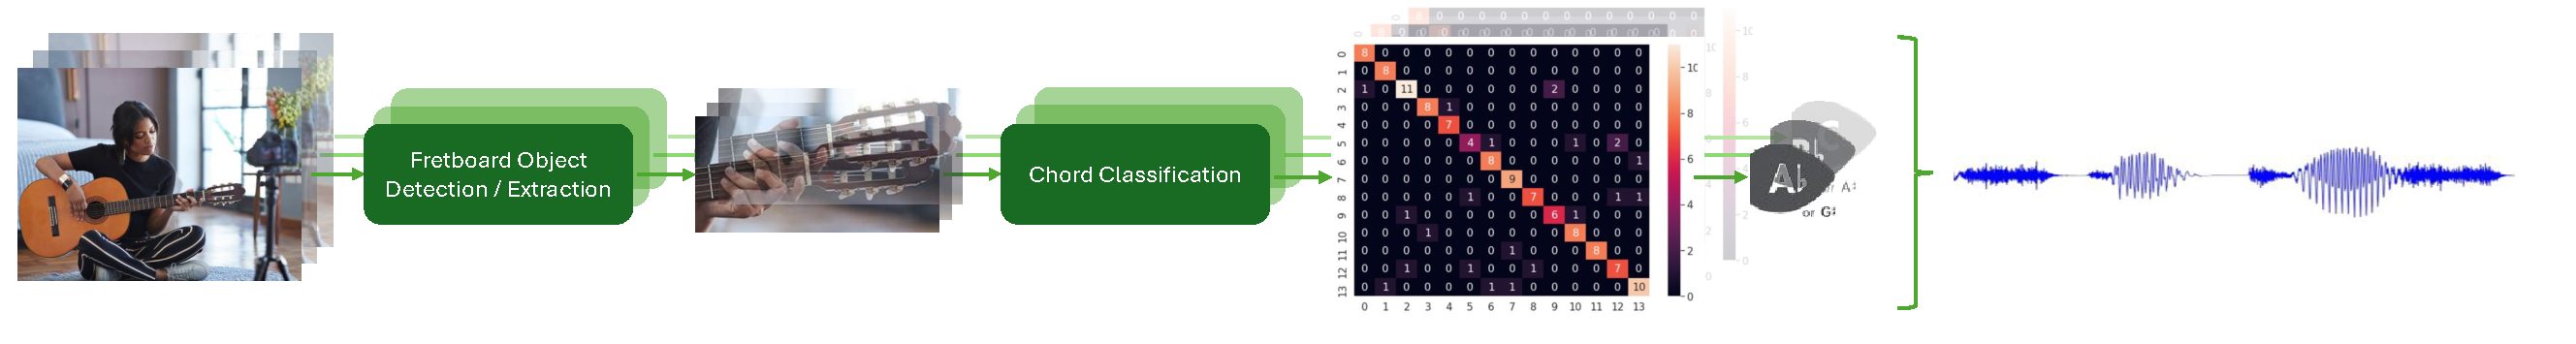
\includegraphics[width=\textwidth]{images/task-diagram.pdf}
    \caption{Overview of the Model, showcasing the 2 most important tasks: 
    Fretboard Detection and Chord Classification, done for each frame of an input video. Image taken from \textit{Getty Stock Images}, confusion matrix image taken from \cite{Kristian_Zaman_Tenoyo_Jodhinata_2024}.}
    \label{fig:model-diagram}
\end{figure*}

\textbf{What challenges do you aim to address in this task?}
\cref{fig:model-diagram} illustrates a bird's eye view of our model architecture. Essentially, we aim to address the following three problems: 
\begin{enumerate}[label=\arabic*)]
    \item \emph{Fretboard Detection}: Given an image or video frame, detect the bounding box that outlines the fretboard.
    \item \emph{Chord Classification}: Given an image or video frame, classify the chord being played.
    \item \emph{Seamless Audio Generation}: Given the chords being played, generate the audio of the music piece.
\end{enumerate}
Y. Kristian et al. \cite{Kristian_Zaman_Tenoyo_Jodhinata_2024} focused on the first two problems, while we aim to address the third problem as well. This is a challenging task since it requires the model to seamlessly generate audio from the classified chords, effectively crossing into the \emph{generative} side of Neural Networks. That is, we aim to move beyong chord classification to also include audio synthesis. In Section \cref{sec:methods} and \cref{sec:datasets}, we briefly cover the methods and datasets we plan to use to address these challenges.

\textbf{What do you want to have completed by the mid-term? E.g., code for the task, data collection, results for baselines, etc.}




\section{Methods}\label{sec:methods}

What models/frameworks do you use to solve the challenges?

Why can the proposed method / analysis solve your problem?

What are the main differences between your method and existing methods (if applicable)?

What is the required computational budget for the training/analysis? (E.g. are you planning on using pretrained backbones?)

\section{Datasets}\label{sec:datasets}

We have chosen the following datasets to train and evaluate our models, depending on the specific task to address: \emph{fretboard detection}, \emph{chord classification}, and \emph{seamless audio generation}. Furthermore, we follow the contributions of Y. Kristian et al. \cite{Kristian_Zaman_Tenoyo_Jodhinata_2024} by first using three different pre-trained datasets to start off our models and leverage transfer learning techniques to improve the overall performance.
\subsection{Pre-trained Datasets}
The chosen datasets have each their own features, thus each one is used to pre-train a specific model.

\begin{enumerate}[label=\arabic*)]
    \item \textbf{ImageNet Dataset}: This dataset is used for pre-training our \emph{guitar chords classifier model}. It has over 14 million images that cover 20,000 types of natural objects \cite{russakovsky2015imagenetlargescalevisual}.
    \item \textbf{COCO Dataset}: This dataset is used for pre-training our \emph{fretboard detection model}. The dataset is of considerable size and is dedicated to object identification. Approximately 200,000 labeled images are organized into 80 distinct categories \cite{lin2015microsoftcococommonobjects}. Although somewhat comparable to ImageNet, the COCO dataset possesses a distinct emphasis.
    \item \textbf{EgoHands Dataset}: Similar to ImageNet, this dataset is also used for pre-training our \emph{guitar chords classifier model}. The dataset includes over 15,000 hand images with high-quality labels \cite{Bambach_2015_ICCV}.
    \item \textbf{GuitarSet}: This dataset is used for pre-training our \emph{seamless audio generation model} from the classified guitar chords. It provides high quality acoustic guitar recordings alongside time-aligned annotations including fret positions, chords, among others \cite{Xi2018}.
\end{enumerate}

A similar technique was used by \cite[2022]{Jadhav_transferlearning} for improving their model's performance by using the ImageNet dataset to pre-train their model and then fine-tuned it using the EgoHands dataset. This approach allowed them to achieve an overall higher accuracy.

\subsection{Fretboard Detection}
This one has both: \cite{guitar-chords-daewp_dataset}. 
Only fretboard: \cite{guitar-ppfil_dataset}, \cite{done-npcll_dataset}.

\subsection{Chord Recognition}
For chord recognition: \cite{guitar-chord-tvon8_dataset}, \cite{guitar-chord-bounding-box_dataset}, \cite{guitar-chord-handshape_dataset}.

\subsection{Seamless Audio Generation}
sdf

\section{Evaluation}

How is your method going to be evaluated?

What metrics are suitable?

Do you need to define your own metric for evaluation?

%%%%%%%%% REFERENCES
{\small
\bibliographystyle{ieee_fullname}
\bibliography{references}
}

\end{document}
